\documentclass[a4paper]{article}

% Packages
\usepackage{amsmath} % For math symbols and equations
\usepackage{amssymb} % For math symbols
\usepackage{enumerate} % For custom numbering of lists
\usepackage{cancel}
\usepackage[
  inner=2cm, % Set inner margin to 2 cm
  outer=2cm, % Set outer margin to 2 cm
  bindingoffset=0.5cm, % Set binding offset to 0.5 cm
  top=2cm, % Set top margin to 2 cm
  bottom=2cm % Set bottom margin to 2 cm
]{geometry}
\usepackage{fancyhdr} % For custom headers and footers
\usepackage{lastpage} % For referencing the last page number
\usepackage{titlesec} % For custom section and subsection headings
\usepackage[version=4]{mhchem} % Required package for chemical equations
\usepackage{hyperref}
\usepackage[
backend=biber,
sorting=anyvt,
style = ieee
]{biblatex} % for using references
\usepackage{parskip}
\usepackage{setspace}
\usepackage{graphicx}
\usepackage{todonotes}
\setuptodonotes{inline}
\usepackage{caption}
\usepackage{adjustbox}
\usepackage{booktabs}
\usepackage{enumitem}

\addbibresource{hw2refs.bib}

% Page setup
\pagestyle{fancy} % Set page style to fancy
\fancyhf{} % Clear default headers and footers
\lhead{Bekir Şahin} % Set left header to your name
\rhead{ENVE422 - Homework 2} % Set right header to assignment name
\cfoot{\thepage\ / \pageref{LastPage}} % Set footer to page number

% custom enumaration
\newlist{sludgenum}{enumerate}{1}
\setlist[sludgenum]{label={\textbf{Sludge \arabic*:}}, align=left, wide = 0pt}

% Section and subsection setup
\titleformat{\section}{\large\bfseries}{Question \thesection}{1em}{} % Set section format
\titleformat{\subsection}{\bfseries}{Part \thesubsection}{1em}{} % Set subsection format
\titlespacing{\section}{0pt}{0.25\baselineskip}{0.25\baselineskip} % Adjust spacing before and after section
\titlespacing{\subsection}{0pt}{0.25\baselineskip}{0.25\baselineskip} % Adjust spacing before and after subsection

% Document information
\title{Department of Environmental Engineering\\Middle East Technical University\\Spring 2023\\ENVE422\\Treatment and Disposal of Water \& Wastewater Sludges\\Homework 2 Submission} % Set document title
\author{\href{sahin.bekir@metu.edu.tr}{Bekir Şahin}} % Set document author
\begin{document}
\setcounter{page}{0}
\onehalfspacing
\maketitle % Add title to document
\thispagestyle{empty}
\listoftodos
\newpage
\todo{Grammarly check}
\section{}
\todo{Formulas are okay, check the numbers and the description once more to polish}
A mass balance for completely mixed continuous aerobic digester \autocite{metcalf2014} can be written as:
\begin{equation}
    \text{Input} - \text{Output} - \text{Change in reactor} = \text{Net Change} \label{eq:massbalance}
\end{equation}
\begin{minipage}[c]{0.5\textwidth}
Using the Equation \ref{eq:massbalance}, the following mass balance can be written:
$$\frac{dS}{dt}*V = Q_{in} S_{in} - Q_{out} S + V r$$
$$r = -K_dS$$
All sides are divided by the volume:
$$\cancelto{\text{0 since SS}}{\frac{dS}{dt}} = \frac{Q_{in} S_{in}}{V} - \frac{Q_{out} S}{V} - K_dS$$
Since there is no change in flow, both can be notated by $Q$:
$$0 = \frac{Q S_{in}}{V} - \frac{Q S}{V} - K_d S$$
\end{minipage}
\hfill
\begin{minipage}{0.4\textwidth}
\fbox{\parbox{0.95\textwidth}{\textbf{Assumptions}\\Aerobic digestion\\Completely mixed, continuous flow\\Steady state\\Fixed volume ($V$)\\$Q_{in} = Q_{out}$\\$K_d = 0.1 \text{ day}^{-1}$}}
\end{minipage}
\begin{equation}
    V = \frac{Q (S_{in} -  S)}{K_d S } \label{eq:volume}
\end{equation}
Since we know the daily flow rate and daily loading rate, we can calculate the desired effluent concentration. With 50\% VSS reduction, the effluent concentration is $\mathbf{41\frac{2}{3}}$ kg/m$^3$. Using the Equation \ref{eq:volume}, the volume for the digester can be calculated as follows:
$$V=\frac{500\text{ kg/d}-250\text{ kg/d}}{0.1\text{/d}*41\frac{2}{3}\text{ kg/m}^3}=\boxed{60 \text{ m}^3}$$
\section{}
I HAVE NO IDEA \autocite{vesilind1988}\todo{Q2 - Find a solution to this problem}\todo{Q2 - Maybe check the reference?}\todo{Q2 - There is a part in Metcalf but no designing procedure}
Woodchips -> movement of air by forming passages, dropping moisture content, 
the sludge is not agitated
nutrient is the most ipmortant parameter C/N 20:1 at least
moisture should be higher than 40\% but not higher than 60\% since it creates anaerobic clumps
availability of minewrals, pH and oxygen availability are the other operational parametes
windrow wide 2.5 m and hight 1-2m

\section{}
The given shear stress (Pa) and shear rate (1/s) are tabulated in Table \ref{tab:rheology} and scatter plotted with different shapes and shades on Figure \ref{fig:SludgeShear}.
\begin{table}[ht]
    \caption{Shear stress (N/m$^2$) and shear rate (1/s) values for Sludge 1, Sludge 2 and Sludge 3}
    \centering
    \begin{tabular}{cccccc}
         \toprule
         \multicolumn{2}{c}{\textbf{Sludge 1}} & \multicolumn{2}{c}{\textbf{Sludge 2}} & \multicolumn{2}{c}{\textbf{Sludge 3}} \\
         \cmidrule(lr){1-2} \cmidrule(lr){3-4} \cmidrule(lr){5-6}
         Shear Stress & Shear Rate & Shear Stress & Shear Rate & Shear Stress & Shear Rate \\
         N/m$^2$ & s$^{-1}$ & N/m$^2$ & s$^{-1}$ & N/m$^2$ & s$^{-1}$ \\
         \cmidrule(lr){1-1} \cmidrule(lr){2-2} \cmidrule(lr){3-3} \cmidrule(lr){4-4} \cmidrule(lr){5-5} \cmidrule(lr){6-6}
         3.8	& 1.8	& 1.7	& 1.8	& 15.4	& 1.8 \\
         5.4	& 3.7	& 3.6	& 3.7	& 17.3	& 3.7 \\
         9.0	& 7.3	& 7.5	& 7.3	& 21.3	& 7.3 \\
         14.1 & 14.7	& 15.0	& 14.7 & 28.7 & 14.7 \\
         23.1 & 36.7 & 36.9 & 36.7 & 50.6 & 36.7 \\
         35.7 & 73.4 & 74.2 & 73.4 & 87.9 & 73.4 \\
         \bottomrule
    \end{tabular}
    \label{tab:rheology}
\end{table}
\begin{sludgenum}
    \item \textsl{Shear thinning} behavior can be expressed as curves starting from the origin and concave upwards as shear rate increases; that is, shear rate increases less proportional to shear stress \autocite{Rao2014}. This type of fluids are called \textit{pseudoplastic} fluids. The shear breaks down the structures in the fluid, making it a thinner complex \autocite{sanin2011, dick1967}.\\
    Performing a power series regression for Sludge 1 values results in 0.95 as the intercept and 0.61 as the slope with 0.9977 $R^2$ value. Thus, Sludge 1 is categorized as \textbf{pseudoplastic fluid}.
    \item For the case of \textsl{Newtonian} fluids, the shear rate and shear stress are directly proportional to each other and the plotting begins from the origin \autocite{Rao2014}.\\
    If the Sludge 2 values are checked, it can be seen that this is the case. A linear regression for that sludge shear rates and shear stresses yields intercept as -0.03 and the slope as 1.01 with $R^2$ equaling to 1. Since the intercept value is really close to 0, the intercept can be regarded as 0. Therefore, Sludge 2 shows \textbf{Newtonian} characteristics.
    \item In cases where the flow does not start until a threshold shear stress value, followed by a straight line follows \textsl{Bingham plastic} model \autocite{Rao2014}.\\
    The linear model conducted for Sludge 3 gives the intercept as 13.70 and the slope as 1.01 with $R^2$ value of 1. As a result, the Sludge 3 follows \textbf{Bingham plastic} model.
\end{sludgenum}
\begin{figure}[ht]
    \centering
    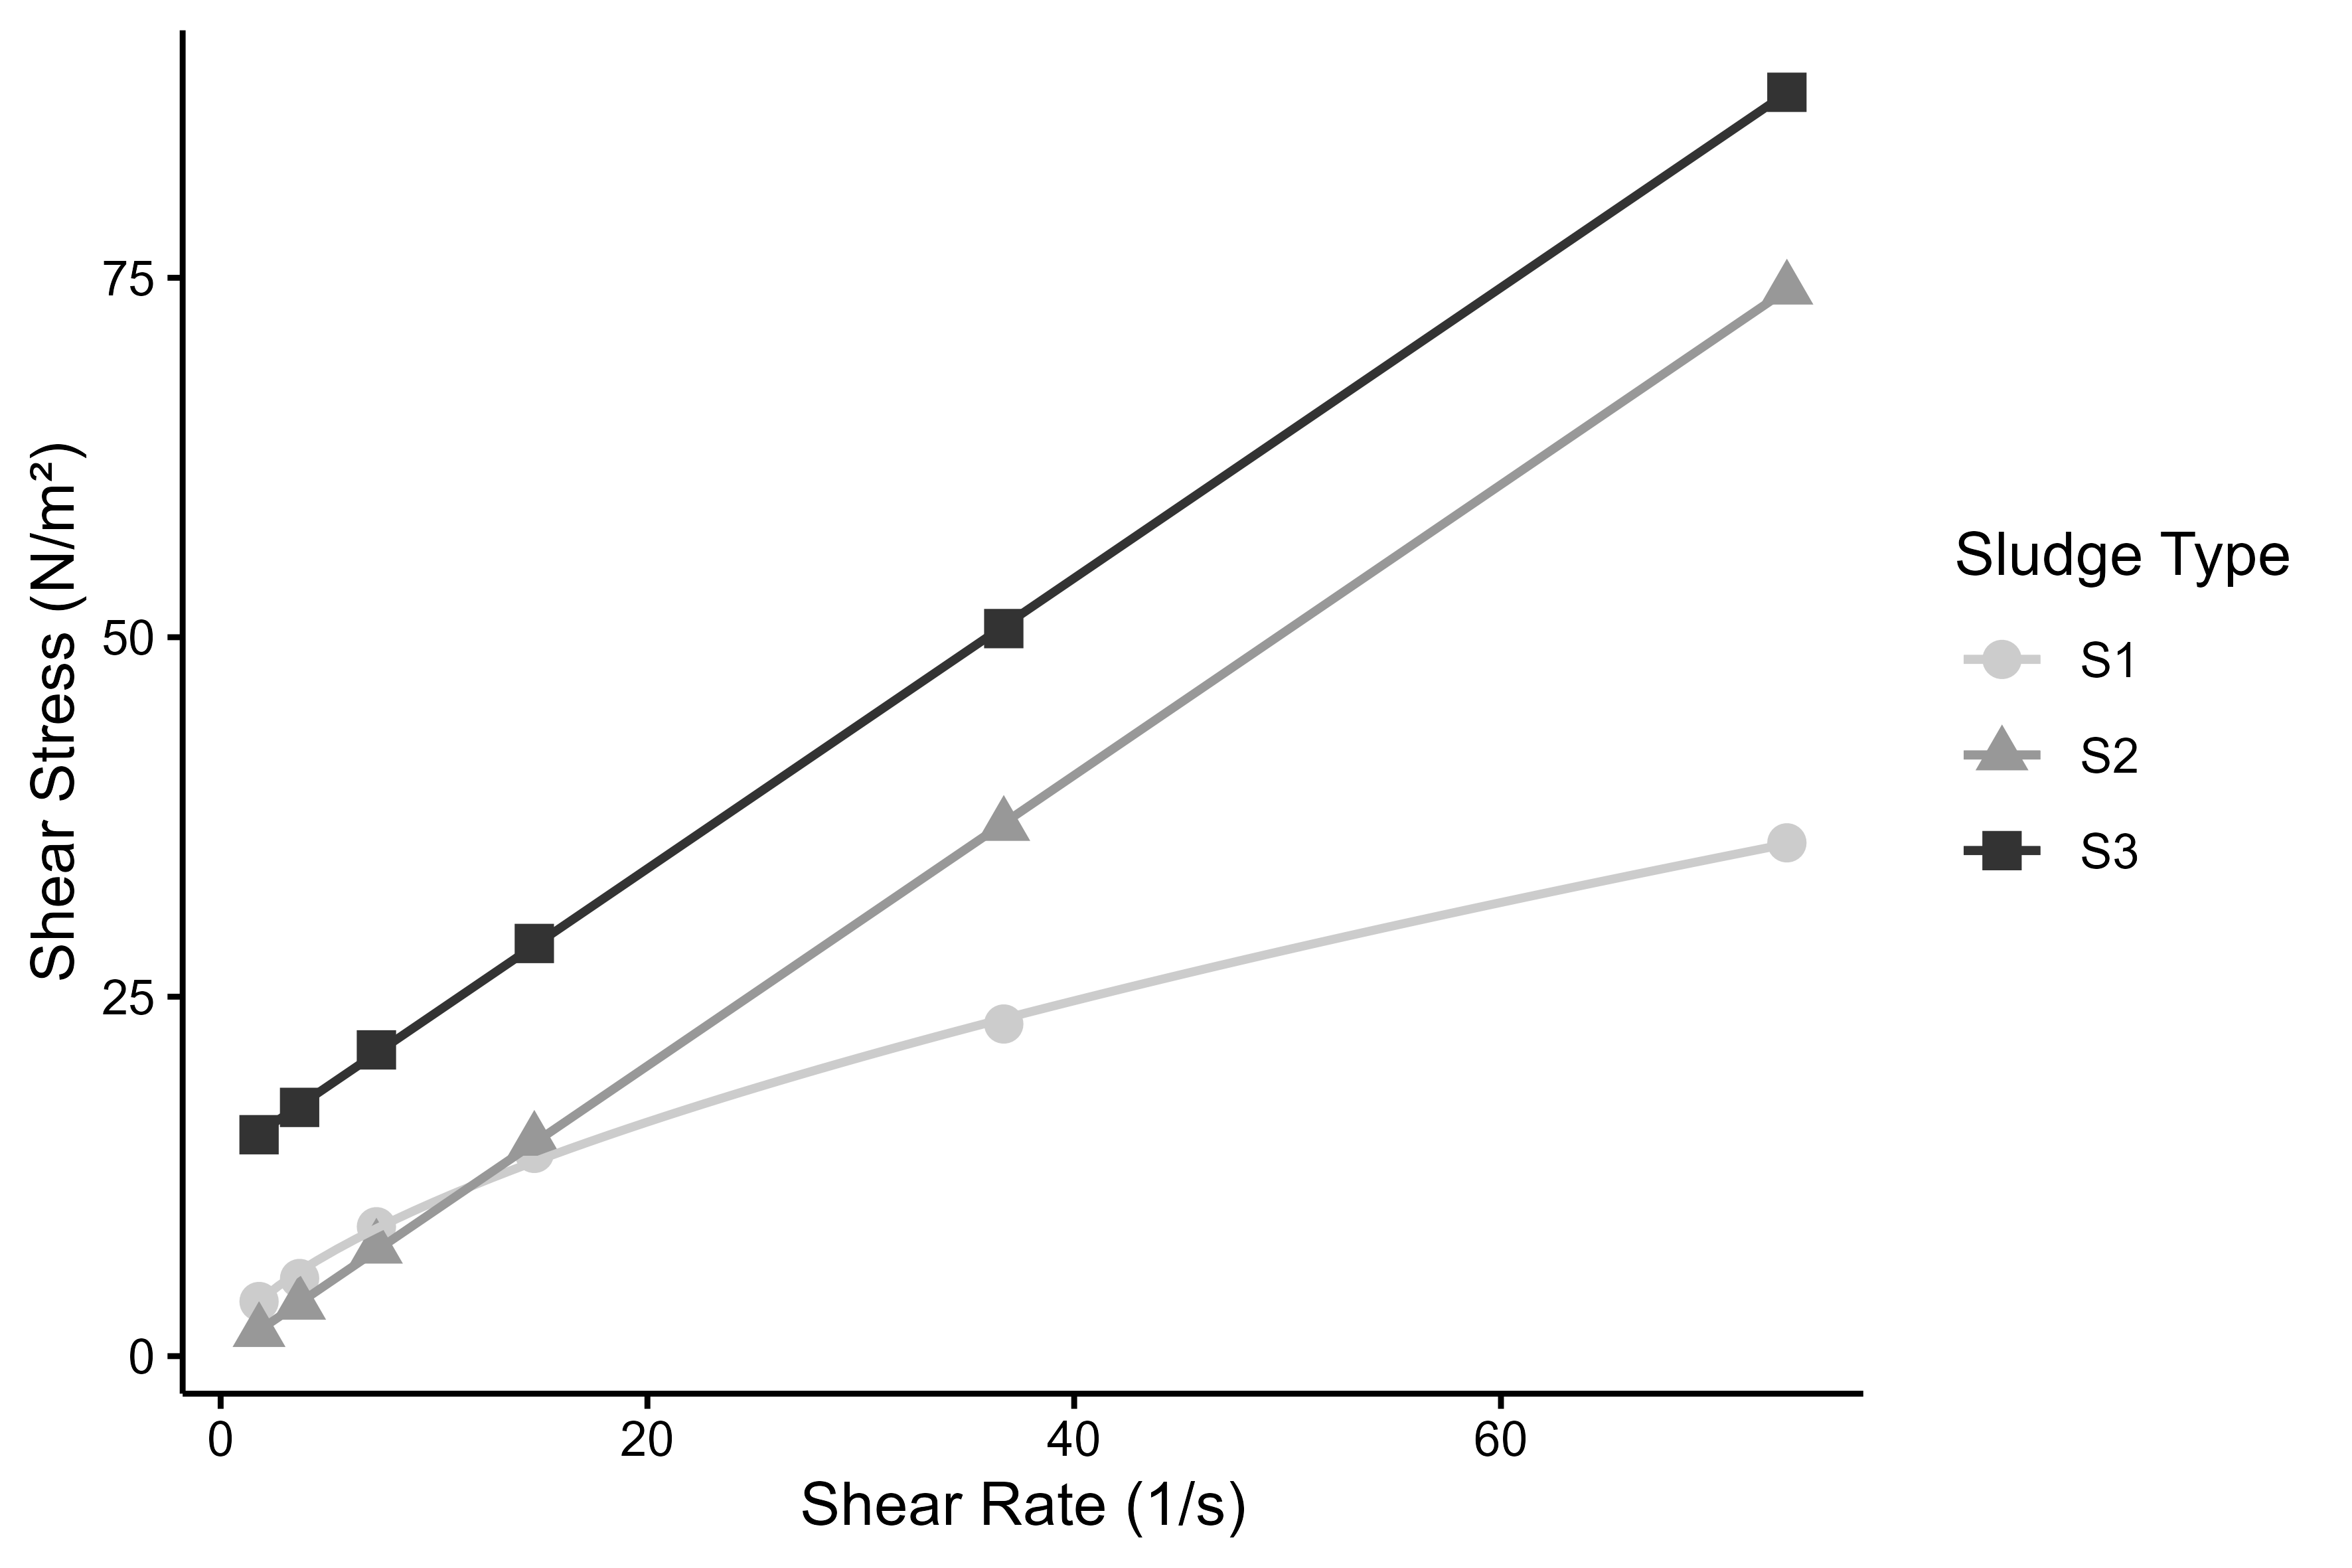
\includegraphics[scale=1]{homeworks/hw2/sludgeShear.png}
    \caption{Sludge rheology for 3 types of sludges}
    \label{fig:SludgeShear}
\end{figure}
The summarized version of the values for rheology models plotted with lines in Figure \ref{fig:SludgeShear} are given in the Table \ref{tab:finalized}.
\begin{table}[ht]
    \centering
    \caption{The sludge analysis summary}
    \begin{tabular}{cccccc}
    \toprule
    \textbf{Sludge \#} & \textbf{Model Formula} & \textbf{Slope} & \textbf{Intercept} & \boldmath{$R^2$} & \textbf{Sludge Type} \\
    \midrule
    Sludge 1 & $\ln(y) = m\ln(x) + b$ & 0.61206 & 0.95382 & 0.9977 & \textsl{Pseudoplastic Fluid} \\
    Sludge 2 & $y = mx + b$ & 1.01075 & -0.02996 & 1.0000 & \textsl{Newtonian Fluid} \\
    Sludge 3 & $y = mx + b$ & 1.01035 & 13.69598 & 1.0000 & \textsl{Bingham Plastic Fluid} \\
    \bottomrule
    \end{tabular}
    \label{tab:finalized}
\end{table}
\section{}
\begin{minipage}[c]{0.5\textwidth}
Since there is no information on the flow rate for the raw sludge, \textbf{velocity}, \textbf{C} and \textbf{S} in the SI Hazen–Williams formula (\ref{eq:H-W}) are missing. In this case, an empirically derived graph such as Figure 4.2 (pg. 120) in \autocite{sanin2011} can be used to determine the energy gradient for further estimation.\\Due to the fact that the sludge is different in terms of solids concentration, considering it causing more head loss in the pipe, an altered C value should be used for any pipe while pumping sludge. Such modification can be applied for a pipe with C value of 100 \autocite{brisbin1957}.
\end{minipage}
\hfill
\begin{minipage}{0.4\textwidth}
\fbox{\parbox{0.95\textwidth}{\textbf{Assumptions}\\Solid concentration = 4\%\\Full pipe, pressurized flow\\No exit or minor losses\\Turbulent Flow\\No thixotropic behavior\\Not obstructed pipe\\Hazen–Williams Equation}}
\end{minipage}
\begin{equation}
    v=0.85*C*R^{0.63}*S^{0.54} \label{eq:H-W}
\end{equation}
Assuming v = 1.22 m/s (4 ft/s) with 4\% solid concentration yields:\\
$S = 0.04$\\
Using Table \ref{tab:H-WCoeffs}, 4\% solid concentration results in C with the value of 61.
$1.22=0.85*61*R^{0.63}*0.04^{0.54}$
\begin{table}[ht]
    \centering
    \caption{Hazen–Williams Coefficients for Various Solids Concentrations of Raw Sludge \autocite{brisbin1957}}
    \begin{tabular}{cc}
    \toprule
    Percent Total Solids & Apparent H-W Coefficient, Based on C = 100 for Water \\
    \midrule
    0 & 100 \\
    2 & 81 \\
    \textbf{4} & \textbf{61} \\
    6 & 45 \\
    8.5 & 32 \\
    10 & 25 \\
    \bottomrule
    \end{tabular}
    \label{tab:H-WCoeffs}
\end{table}
\newpage
\printbibliography
\end{document}